\chapter{Conclusion}

\label{ch:conclusions}

\section{Summary of Thesis Achievements}
% In this thesis, we have proposed several approaches to improve the sample efficiency of deep reinforcement learning (DRL) in tasks with sparse and delayed rewards. Moreover, we provide a comprehensive quantitative and qualitative analysis on the agents trained with and without domain randomisation (DR) to visualise and explain why DR can improve the robustness of the agents against unseen scenarios. 
In this thesis, in order to improve the sample efficiency of deep reinforcement learning (DRL) in the environments with sparse or delayed rewards, three novel DRL methods are proposed. In these methods, we propose 1) a novel self-imitation learning loss term that allows the agent to overcome hard exploration problems by using hindsight experiences, 2) a novel sampling strategy that increases the chance to sample valuable transitions for the training and 3) a diversity-based intrinsic reward that can provide auxiliary dense feedback to the agent for helping the exploration in the environments with delayed or sparse rewards. From extensive experiments, these methods achieve better performance than other baseline approaches when using the same number of samples for training, which demonstrates that our methods indeed improve the sample efficiency of DRL algorithms. Moreover, we provide a comprehensive quantitative and qualitative analysis on the agents trained with and without domain randomisation (DR) to visualise and explain why DR can improve the robustness of the agents against unseen scenarios.

Firstly, in \textbf{Chapter}~\ref{ch:drl_interp}, we investigate the agents trained with and without DR to interpret why the agents trained with DR are more robust to unseen scenarios. In this work, we built two simulated robot environments that provide both visual and proprioceptive inputs. The agents are trained to manipulate the robot arm to reach a specific target with different training conditions (different types of inputs and with or without DR). In order to analyse the trained agents, various previously unseen test conditions are used to evaluate the robustness of the trained agents, and both quantitative and qualitative analysis are applied to provide sufficient insights into the behaviour of the trained agents. We further propose an improved occlusion-based saliency map method to provide better attention maps of the agents at each timestep. From results, we show that the DR agents have better generalisation ability to local visual changes, and also exhibit a degree of robustness to global visual changes. The saliency maps of the DR agents focus more on the target object, while non-DR agents show attention to the distractors. In the layer re-initialisation, DR agents also show significant changes in the parameters, which leads to more robust features. The recurrent ablations also reflect that LSTM is only necessary when DR is activated. In the end, some recommendations for applying interpretability methods to DRL agents are also suggested. 

Secondly, in \textbf{Chapter}~\ref{ch:esil} and \textbf{Chapter}~\ref{ch:dtgsh}, research aims to improve the sample efficiency of goal-oriented RL in continuous control tasks with sparse rewards. In \textbf{Chapter}~\ref{ch:esil}, a novel self-imitation learning loss is proposed to overcome the difficulty that the agent rarely achieves positive rewards from the environment, where hindsight goal relabelling is leveraged to modify failed trajectories into successful ones. Then, these modified trajectories are used to accelerate the training/exploration in the initial stages of training via a self-imitation learning scheme. In addition, a trajectory selection module and an adaptive weight are proposed to remove redundant hindsight experiences and maintain the balance between the exploration and exploiting. In \textbf{Chapter}~\ref{ch:dtgsh}, it can be argued that when using hindsight goal relabelling, not all agent's experiences contribute equally to the training, and the naive uniform sampling may lead to inefficient learning. In order to achieve valuable experience, a more efficient sampling strategy is introduced. We first sample trajectories according to the diversity of the goal states as modelled by determinantal point processes (DPPs). Then, transitions with diverse goal states are selected from the trajectories by using $k$-DPPs. Extensive experiments in these two chapters demonstrate the effectiveness of our methods and show that our methods achieve state-of-the-art results on several simulated robot manipulation tasks.

Finally, in \textbf{Chapter}~\ref{ch:daim}, diversity is again used via a mechanism of intrinsic motivation, a diversity-augmented intrinsic motivation is proposed to encourage the agent keep exploring novel states in the environment. This intrinsic reward is formulated based on the diversity of adjacent states, measured under the framework of DPPs. Furthermore, a bi-level optimisation is used to guarantee that when increasing the intrinsic reward to encourage the agent to explore novel states, the extrinsic returns are still maximised. Experimental results show that this method outperforms other baselines on the MuJoCo continuous control tasks with standard and delayed reward settings, and it accelerates exploration in the initial stage of training in the arcade learning environments. 
%\section{Applications}

%Applications.
\section{Future Work and Potential Applications}
The topic of my thesis focuses on improving sample efficiency in DRL and interpretability in DRL. Thus, this section can be split into two branches: 1) discussion of limitations and potential extensions to the proposed methods. 2) potential applications to solve scientific problems.

\subsection{Limitations and Extensions}
In \textbf{Chapter}~\ref{ch:drl_interp}, the current work focuses solely on the analysis of visual domain randomisation. In the future, we will also analysis the trained agents with dynamic DR (e.g., changing the frictional coefficient.). Furthermore, instead of using a simple reach task as the test environment, we will further develop more complicated tasks for analysing, such as a stacking cube task or a pick and place task, which are more in line with real-world applications. Another direction for the future is to apply the related interpretability methods to our proposed methods in other chapters and then compare the results with the PPO algorithm, because the learned features and policies may have changed and thus some interesting findings may be obtained to explain why these methods can improve the performance of vanilla PPO algorithm.

In \textbf{Chapter}~\ref{ch:esil}, the proposed episodic self-imitation learning (ESIL) allows on-policy DRL algorithms (e.g., PPO) and hindsight experience replay (HER) to be combined and can be used to solve continuous control tasks with the sparse rewards. However, this still require more samples for training than off-policy DRL algorithms (e.g., DDPG+HER). One possible future study is to improve the sample efficiency with ESIL. Another future work could incorporate self-imitation learning mechanisms with DDPG+HER. Nair \textit{et al.}~\cite{nair2018overcoming} have already done relevant work, where they collect expert demonstrations for imitation learning. Instead of manually collecting demonstrations, a potential improvement is to utilise past good trajectories for self-imitation learning in the off-policy DRL paradigm.

In \textbf{Chapter}~\ref{ch:dtgsh}, the diversity-based sampling strategy is only applicable to environments that contain manipulable objects, such as picking and placing a cube at a target position. In the future, we can extend this method to more general goal-oriented tasks, such as navigating an agent to arrive at a target location in a maze~\cite{florensa2018automatic}.

In \textbf{Chapter}~\ref{ch:daim}, the proposed diversity-augmented intrinsic motivation (DAIM) achieves limited performance in the arcade learning environment (ALE), and it is also unable to address hard exploration tasks, such as Montezuma's Revenge. Therefore, tackling such challenging hard exploration tasks is a potential direction for improvement. One possible solution is to combine the proposed self-imitation loss in Chapter~\ref{ch:esil} with the diversity-based intrinsic reward to enhance the exploration in the above challenging hard exploration tasks.

In addition, although there exists plentiful methods to improve sample efficiency in DRL. However, sample efficiency in DRL is still a challenging problem. Therefore, I will further discuss some interesting and novel directions for my future research work.

Firstly, rather than using HER to address goal-oriented RL problems, C-learning~\cite{eysenbach2020c} provides a new paradigm to solve goal-oriented RL by estimating the probability density over future states. In practice, estimating the probability density function is very difficult, and C-learning estimates this density function indirectly via training a binary classifier to predict if the current state--action pair can generate a specific future state (i.e. the goal state) in the current episode, and the state--action pair has a higher probability of generating the goal state will be assigned with a higher return for training. Extensive experiments also show that C-learning outperforms other baselines in various goal-oriented tasks. Therefore, C-learning provides a new way to solve goal-oriented RL, and it deserves further investigation.

Another way to improve sample efficiency in DRL is to reuse prior knowledge to solve previously unseen tasks. This kind of method can differ from imitation learning methods~\cite{bojarski2016end,xu2017end,torabi2018behavioral} which require collecting demonstrations from the same task. Some related methods like meta-learning based RL~\cite{duan2016rl,wang2017learning,finn2017model} and meta-imitation learning~\cite{duan2017one,finn2017one,huang2019continuous} try to leverage prior knowledge to accelerate the learning of new tasks. Another interesting method called prior accelerated reinforcement (PARROT)~\cite{singh2020parrot}, first pretrains a flow-based generative model that maps the latent variables, which are conditioned on the current state, to an action by using expert demonstrations. Subsequently, this pretrained generative model can be used as a behaviour prior to facilitate the exploration in the new tasks. Thus, how to efficiently reuse prior knowledge/skills is an interesting research topic in the future.

\subsection{Potential Applications}
\begin{figure}[h]
  \begin{subfigure}[t]{0.24\textwidth}
    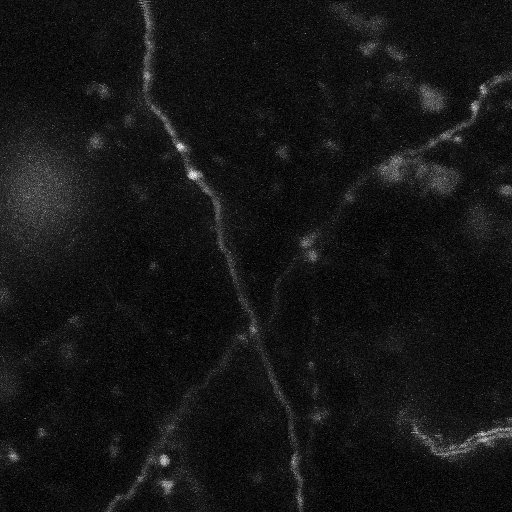
\includegraphics[width=\textwidth]{figures/conclusion/real_img.jpg}
    \caption{Microscopy Image}
    \label{subfig:real_img}
  \end{subfigure}\hfill
  \begin{subfigure}[t]{0.24\textwidth}
    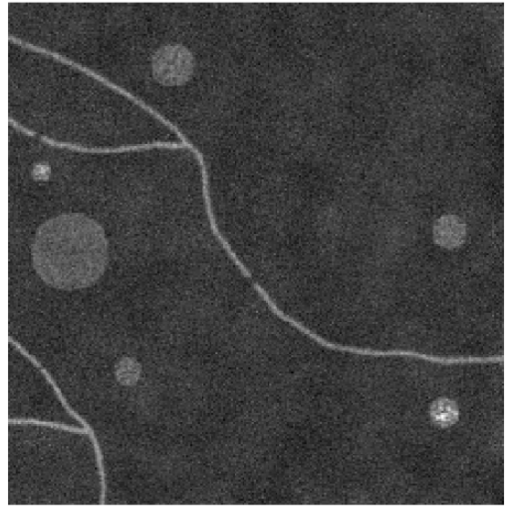
\includegraphics[width=\textwidth]{figures/conclusion/synthetic_image_resize.png}
    \caption{Synthetic Image A}
    \label{subfig:synthetic}
  \end{subfigure}\hfill
  \begin{subfigure}[t]{0.24\textwidth}
    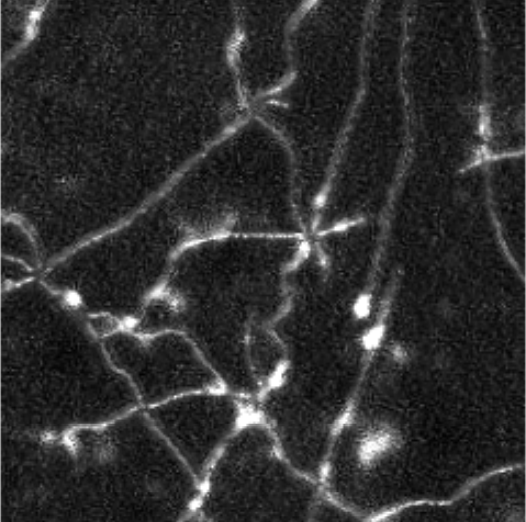
\includegraphics[width=\textwidth]{figures/conclusion/CapGAN.png}
    \caption{Synthetic Image B}
    \label{subfig:synthetic_b}
  \end{subfigure}\hfill
  \begin{subfigure}[t]{0.24\textwidth}
    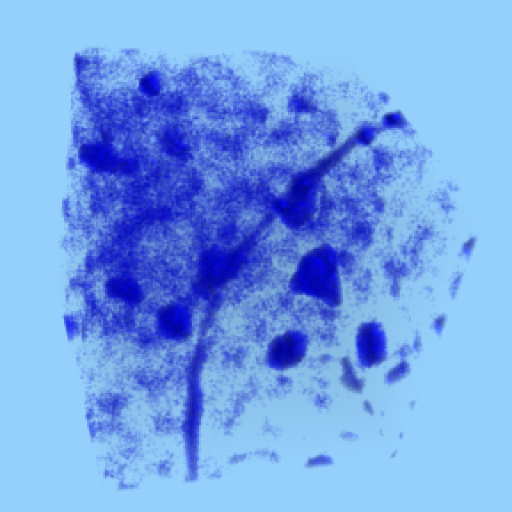
\includegraphics[width=\textwidth]{figures/conclusion/3d_resize.png}
    \caption{3D Synthetic Image}
    \label{subfig:3d_synthetic}
  \end{subfigure}\hfill
  \caption[Examples of different types of axon images.]{Examples of different types of axon images. (a) is a real microscopy image, (b) is the basic 2D synthetic axon image, (c) is the 2D synthetic axon image generated by CapsPix2Pix~\cite{bass2018image}, and (d) is the 3D synthetic axon image.} 
  \label{fig:axon_env}
\end{figure}
The recent successful achievement of machine learning for science is AlphaFold~\cite{jumper2021highly}, which leverages state-of-the-art deep learning based techniques to predict the 3D structure of a protein based solely on its genetic sequence, and the predicted structures are far more accurate than the outputs of any previous approaches. Predicting protein structures is important to understand the functionality of proteins in any biological system as well as in the diagnosis and treatment of especially genetic diseases (e.g., Alzheimer). Thus, it is meaningful if DRL can be applied to address some real-world/scientific problems. One potential application of DRL is to track the elongated structure in biomedical/microscopy images, such as axons and blood vessels. 

Automatically tracking elongated structures is a challenging problem in the field of biomedical imaging. In contrast to segmentation, tracking also allows the establishment of correspondences and state estimation to be performed. Some existing algorithms, such as Kalman filtering, particle filtering, or semi-heuristic connectivity algorithms, require tuning parameters manually for different datasets. To alleviate the need for hand-engineering trackers for different biomedical image datasets, we
first formulate the task of tracing paths along the centrelines of elongated structures as a RL problem, and then explore the use of DRL to train deep convolutional neural networks (CNNs) to learn tracking policies. Up to now, we have developed a simulated environment that can generate synthetic axon images with customised settings, such as the number of axons, the number of branches, and the type of noise (see Figure~\ref{subfig:synthetic}). To reduce the reality gap between the real microscopy image (see Figure~\ref{subfig:real_img}) and the synthetic image, we have proposed CapsPix2Pix~\cite{bass2018image} to generate more realistic synthetic images (see Figure~\ref{subfig:synthetic_b}). We have proposed two DRL trackers~\cite{dai2019deep,balaram2019maximum} which are able to solve 2D axon tracking and achieve comparable results with state-of-the-art axon tracking method -- Vaa3D~\cite{peng2010v3d}. However, the above DRL trackers do not yet scale to the 3D axon tracking task (see Figure~\ref{subfig:3d_synthetic}), because they lack effective exploration in the environment. In the future, we will apply different techniques (e.g., intrinsic motivation) to overcome the exploration problems in the 3D tracking task.
%Thus, the intrinsic motivation method can be combined with the DRL tracker, which encourages the agent to explore novel states to find a promising policy and solve the problem.

%Preliminary Results and Future Work.
